\documentclass[a4paper,10pt]{article}
\usepackage[utf8]{inputenc}
\usepackage{amsmath}
\usepackage{hyperref}
\usepackage{fancyhdr}
\usepackage{graphicx}
\usepackage{fancyvrb}
%\usepackage{listings} % for source code
\pagestyle{fancy}

%generate mono-spaced
\def\code#1{\texttt{#1}}

\rhead{}
\lfoot{noise}
\cfoot{}
\rfoot{\thepage}
\renewcommand{\footrulewidth}{0.4pt}
%opening
\title{Generating pleasant noises using microcontrollers}
%\author{Mark Carter \\ email \href{mailto:me@somewhere.com}}
%\author{Mark Carter}
\author{Mark Carter \\ alt.mcarter@gmail.com}
%\author{Mark Carter --- alt.mcarter@gmail.com}

\begin{document}
\maketitle
\thispagestyle{fancy}

\begin{abstract}

A common MCU (microcontrollers) project is the generation of noise for sleep or other purposes. Most projects found on the internet demonstrate how MCUs can be used to generate white noise. However, white noise sounds harsh, or ``tinny'', to humans. Brown noise is more pleasant, but it is difficult to find literature on how to generate it simply.

This paper explains how an approximation to Brown noise can be produced using a cheap MCU, a resistor, and a capacitor. A model and simulation of the underlying electrical theory is presented.
\end{abstract}

\section{Introduction}
Humans hear in the range 20-20kHz \cite{wikihearing}. 
Noise-making machines are often used to promote sleep. They are not particularly cheap, costing around £30 as at July 2019. It is easy to produce white noise using hobbiest MCUs like an Arduino Uno. The following sketch for the Arduino IDE shows just how simple it is:
\begin{verbatim}
void setup() {
  pinMode(12, OUTPUT);
}

void loop() {
  digitalWrite(12, random(2));
}
\end{verbatim} 
The code can be adapted easily to work with a variety of MCUs. Halfacree \cite{halfacree} elaborates on this idea by creating a project called the Sleepduino, consisting of an MCU, a potentiometer, some LEDs and a speaker.  The source file is available on github \cite{sleepduino}. It uses its own algorithm to generate random numbers, although this would not appear to be necessary, as the Arduino IDE already provides a random number generator.

The problem with white noise is that it is unpleasant to human ears. There is too much hissing to it \cite{gulf}, which is caused by the ear's perception of loudness at the higher frequencies. In order to produce a more pleasing sound, the energy output at the higher frequencies needs to be attenuated.

\section{Measurement of sound}

For \emph{power} quantities, a decibel (dB) is defined \cite{dB} as: 
\begin{equation}
 L_P = 10 \log_{10}\left(\frac{P}{P_0}\right)
\end{equation}
where $P$ is the measured power, and $P_0$ is the reference power.

For \emph{field} quantities, such as voltages and amplitudes, it is defined as:

\begin{equation}
 L_F = 10 \log_{10}\left(\frac{F^2}{F^2_0}\right) \equiv 20 \log_{10}\left(\frac{F}{F_0}\right)
\end{equation}

where $F$ is the measured field value, and $F_0$ is the reference field value.

The dB is therefore a relative to some reference value, rather than absolute one. Note that if an amplitude or voltage halves, its dB changes by approximately -6 dB $( = 20 \log_{10}\frac{1}{2})$.

Consider the representation of amplitudes in a sound file, where each sound sample is represented by an unsigned 8-bit byte. Each byte has a minimum value of 0, and a maximum value of 255 inclusive. Choosing $F_0$ to be the value 255, it follows that the dB value for an amplitude of 255 is 0dB. An amplitude of 128, it is approximately half of 255, therefore measures as $\approx$-6dB.

An \emph{octave} refers to the doubling of frequency, whilst a \emph{decade} refers to a ten-fold increase of freuency. Thus, for example, Brownian noise is described as falling 6dB per octave, or 20dB per decade \cite{brown}.


\section{White noise}
This section defines white noise and ...

White noise is a random signal having equal intensity at different frequencies, giving it a constant power spectral density\cite{wiki_white}. Its spectrum looks like this:

\begin{center}
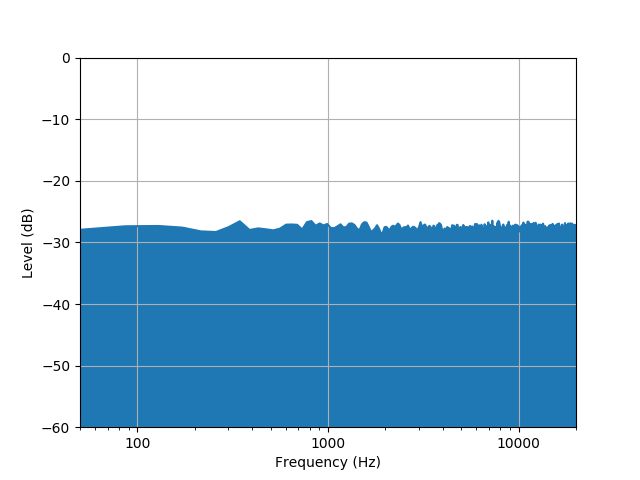
\includegraphics[height=6cm]{white.png}
\end{center}

The following code generates it (\code{white.c}):
\begin{Verbatim}[tabsize=8]
#include <assert.h>
#include <stdio.h>
#include <stdlib.h>

int main()
{
	FILE* fp = fopen("noise.raw", "wb");
	assert(fp);
	for(int i = 0; i<80000; ++i) {
		int v = rand() % 256;
		fprintf(fp, "%c", v);
	}
	fclose(fp);
	return 0;
}
\end{Verbatim}
%\end{lstinputlisting}
%\lstinputlisting[caption=Scheduler, style=customc]{hello.c}

%\lstinputlisting[label=foo, caption=My caption]{white.c}
 
\section{Brown noise}

Bownian noise, also known as red or random walk noise, is coined after Robert Brown, the discoverer of Brownian motion. \cite{brown}. It is obtained as the integral of white noise:

\begin{equation}
 W(t) = \int_{0}^{t} \frac{dW(\tau)}{d\tau} d\tau
\end{equation}

Programmatically:
\begin{equation}
 y_{n} = y_{n-1} + w_n
\end{equation}
where $y$ is the generated signal at each time step, and $w$ is the white noise for that step.

Translated to a C program (\code{brown.c}):
\begin{Verbatim}[tabsize=8]
#include <assert.h>
#include <stdio.h>
#include <stdlib.h>

int main()
{
	const int n = 100 * 1000;
	float y[n];
	y[0] = 0; // the signal
	float min = 0, max = 0;
	for(int i = 1; i< n; ++i) {
		float white = (rand() % 7) - 3;
		y[i] = y[i-1] + white;
		if(y[i]>max) max = y[i];
		if(y[i]<min) min = y[i];
	}

	// output a normalisation of the array
	FILE* fp = fopen("noise.raw", "wb");
	assert(fp);
	for(int i =0; i< n; ++i) {
		int v = 255.0 * (y[i] - min)/(max-min);
		fprintf(fp, "%c", v);
	}
	fclose(fp);

	return 0;
}
\end{Verbatim}
Since the output follows a random walk, it is unbounded in how far it can stray, and therefore must be normalised. A typical amplitude-time plot might look as follows:

\begin{figure}[h]
\centering
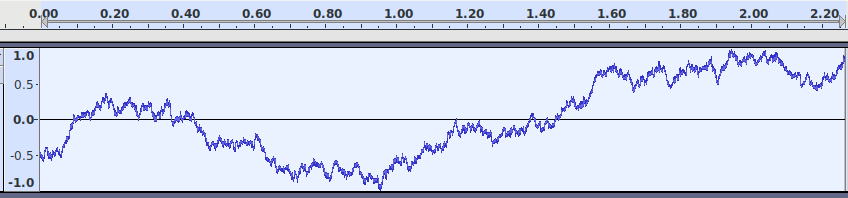
\includegraphics[width=12cm]{brown-amp.png}
\caption{Amplitude against time generated by \code{brown.c}}
\label{fig:brownamp}
\end{figure}

Its frequency spectrum is as follows:
\begin{center}
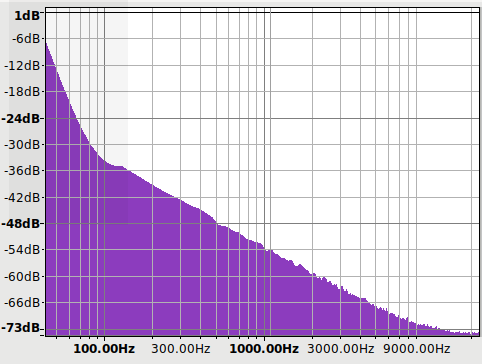
\includegraphics[width=12cm]{brown-freq.png}
\end{center}

This output is not wholly confirmant to a Brown noise signal below about 127Hz, as it attentuates too rapidly at those lower frequencies. Above 127Hz, though, the signal conforms to the property of Brownian noise falling 6dB per Octave, or equivalently 20dB per decade\cite{brown}. For example, at 300Hz, the output is at -42dB, whereas at 600Hz, the output is at -48dB, corresponding to a drop of 6dB per Octave. Equivalently, at 3000Hz, the level is -62dB, corresponding to drop of 20db (=62-42) per decade (3000/300).

Figure \ref{fig:brownamp} shows the presence of long wavelengths (i.e. short frequencies) compared to typical Brownian signal generated by Audacity:
\begin{center}
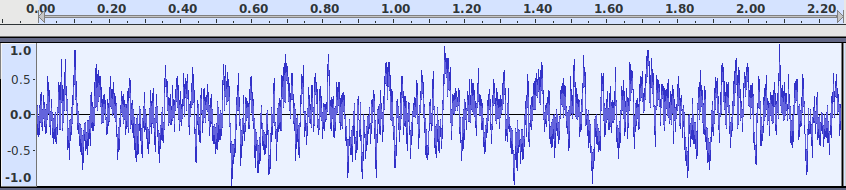
\includegraphics[width=12cm]{brown-amp-audacity.png}
\end{center}

The spectrum is also correct:
\begin{center}
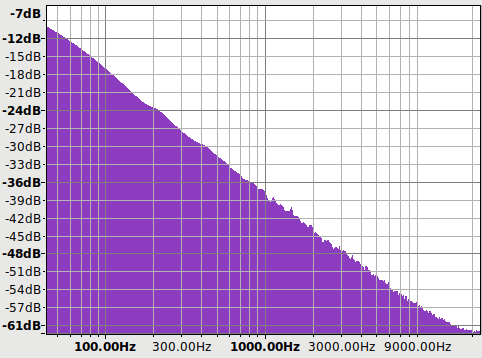
\includegraphics[width=12cm]{brown-freq-audacity.png}
\end{center}
 

\appendix

\section{Appendix: for which no-one has found a use}

Now is the winter of our discontent.
\begin{equation*}
  f(x) = x^2
\end{equation*}

\begin{thebibliography}{9}
 
\bibitem{halfacree}
Halfacree, Gareth.
\textit{Introducing the Sleepduino}
2012 
\\\texttt{https://is.gd/5zEFYt}
Extracted 2 July 2019

 

\bibitem{sleepduino}
Cox, Patrick.
\textit{Basic version of the Sleepduino.}
\\\texttt{https://github.com/patcox/Sleepduino}

\bibitem{gulf}
Gulf Coast Audiology.
\textit{White, Pink or Brown: Which Noise Helps You Sleep Better?}
\\\texttt{https://is.gd/41EOqr}

\bibitem{wikihearing}
Wikipedia.
\textit{Hearing range}
\\\texttt{https://en.wikipedia.org/wiki/Hearing\_range}

\bibitem{wiki_white}
Wikipedia.
\textit{White noise}
\\\texttt{https://en.wikipedia.org/wiki/White\_noise}

\bibitem{wiki_colour}
Wikipedia.
\textit{Colors of noise}
\\\texttt{https://en.wikipedia.org/wiki/Colors\_of\_noise}

\bibitem{audacity}
Audacity.
\textit{Free, open source, cross-platform audio software}
\\\texttt{https://www.audacityteam.org/}

\bibitem{brown}
Wikipedia
\textit{Brownian noise}
\\\texttt{https://en.wikipedia.org/wiki/Brownian\_noise}

\bibitem{dB}
Wikipedia
\textit{Decibel}
\\\texttt{https://en.wikipedia.org/wiki/Decibel}

\end{thebibliography}


\end{document}
